\documentclass{standalone}
\usepackage{tikz}
\usetikzlibrary{patterns, positioning}
\usetikzlibrary{shapes.misc}
\usepackage[outline]{contour}
\contourlength{1.5pt} 
\usepackage[sfdefault]{ClearSans} %% option 'sfdefault' activates Clear Sans as the default text font
\usepackage[T1]{fontenc}

\begin{document}
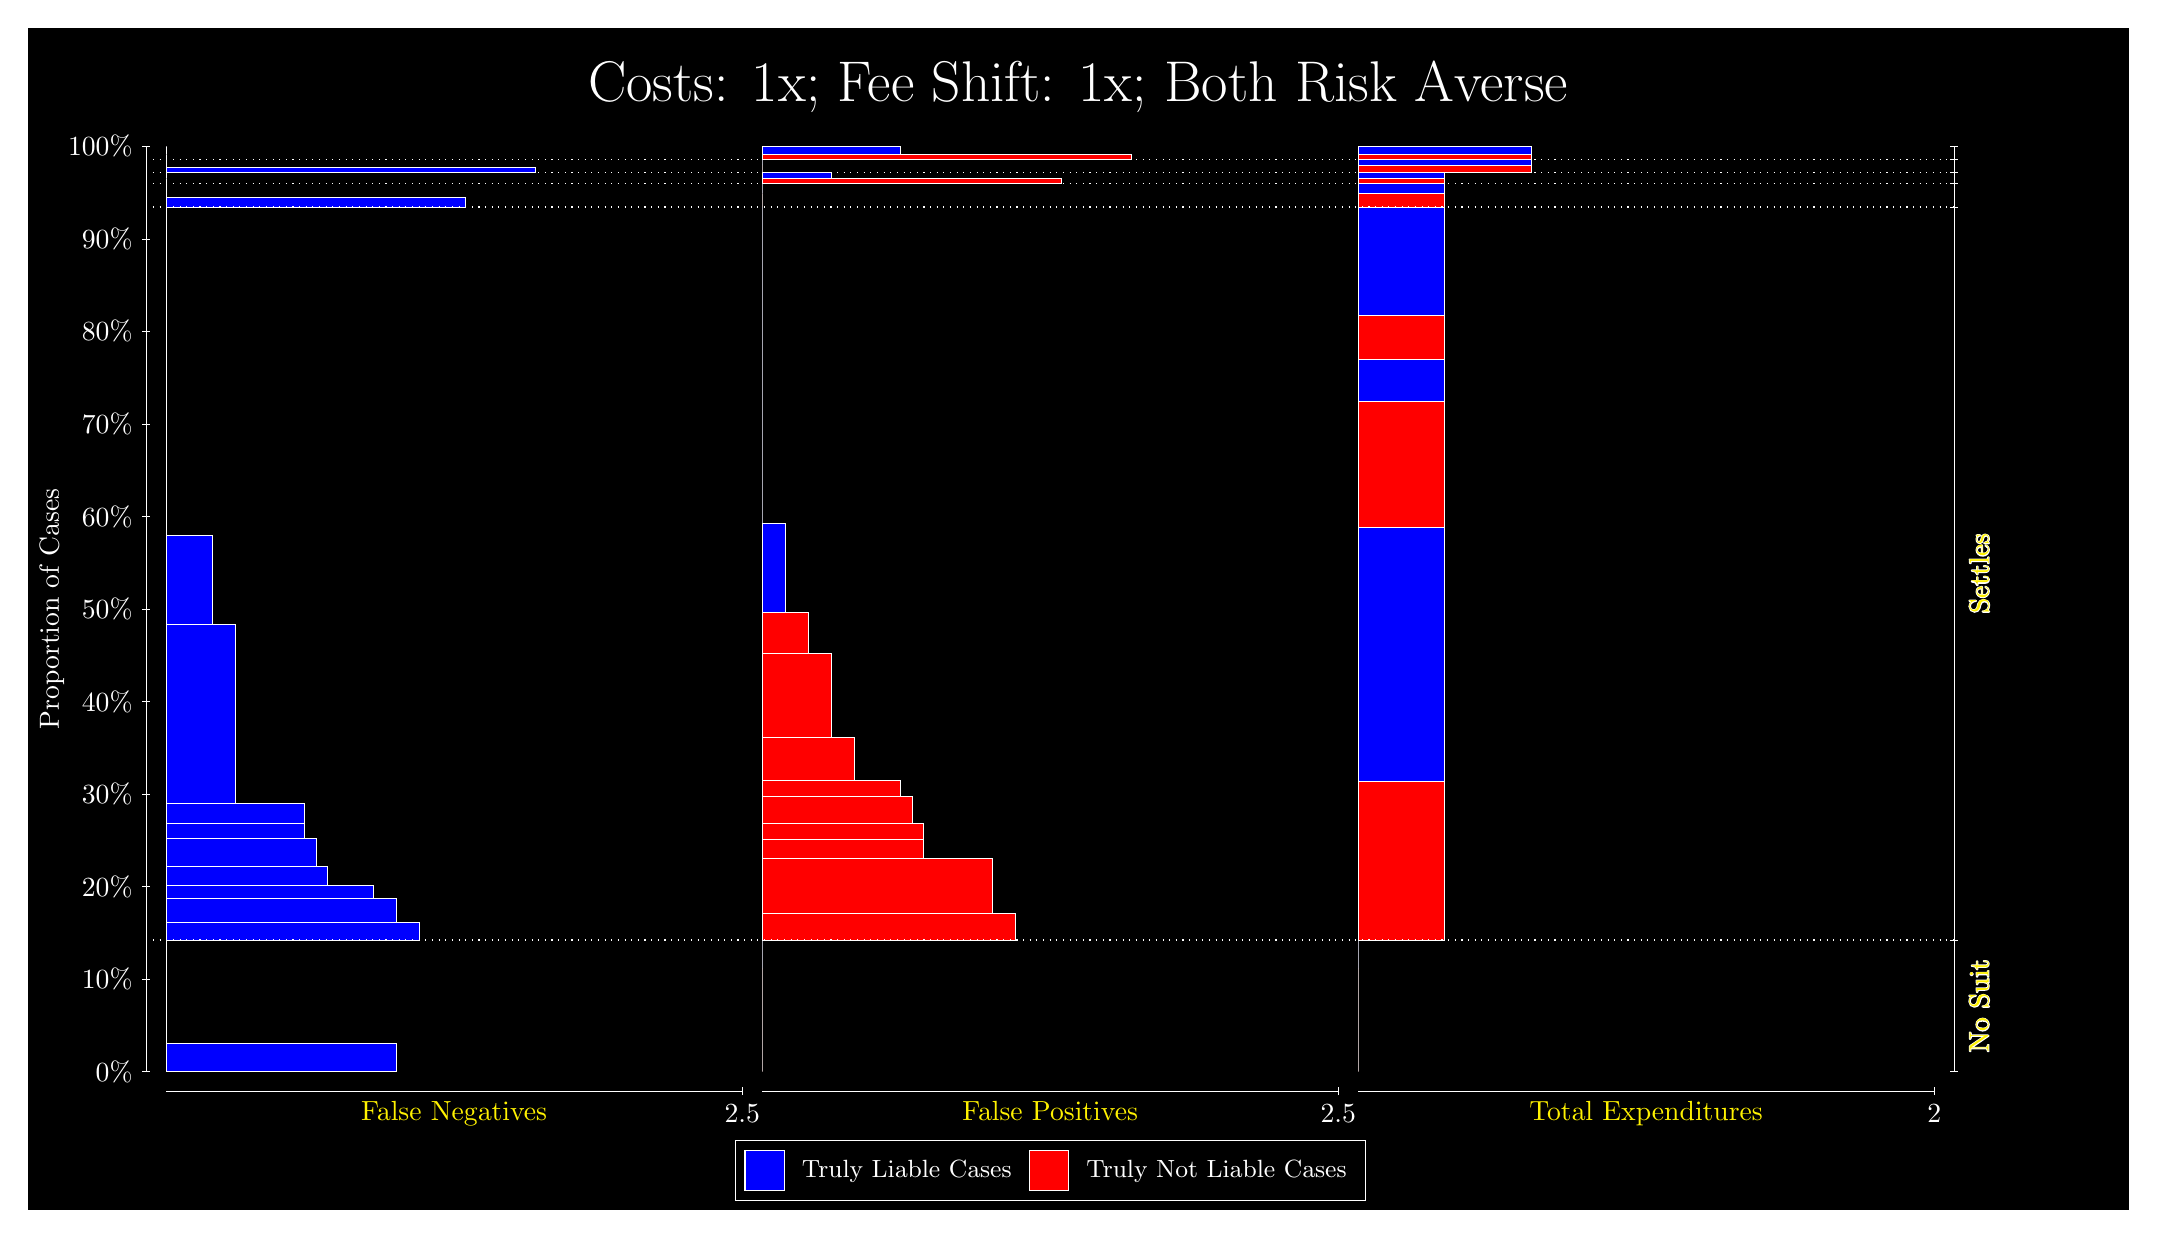
\begin{tikzpicture}
\draw[fill=black] (0,0) rectangle (26.667,15);
\draw[text=white] (0,13.5) rectangle (26.667,15) node[midway] {\huge Costs: 1x; Fee Shift: 1x; Both Risk Averse};
\draw[white, very thin] (1.5,1.75) -- (1.5,13.5);
\node[rotate=90, text=white, anchor=center] at (0.3, 7.625) {Proportion of Cases};
\draw[white, very thin] (1.45,1.75) -- (1.55,1.75);
\node[text=white, anchor=east] at (1.45, 1.75) {0\%};
\draw[white, very thin] (1.45,2.925) -- (1.55,2.925);
\node[text=white, anchor=east] at (1.45, 2.925) {10\%};
\draw[white, very thin] (1.45,4.1) -- (1.55,4.1);
\node[text=white, anchor=east] at (1.45, 4.1) {20\%};
\draw[white, very thin] (1.45,5.275) -- (1.55,5.275);
\node[text=white, anchor=east] at (1.45, 5.275) {30\%};
\draw[white, very thin] (1.45,6.45) -- (1.55,6.45);
\node[text=white, anchor=east] at (1.45, 6.45) {40\%};
\draw[white, very thin] (1.45,7.625) -- (1.55,7.625);
\node[text=white, anchor=east] at (1.45, 7.625) {50\%};
\draw[white, very thin] (1.45,8.8) -- (1.55,8.8);
\node[text=white, anchor=east] at (1.45, 8.8) {60\%};
\draw[white, very thin] (1.45,9.975) -- (1.55,9.975);
\node[text=white, anchor=east] at (1.45, 9.975) {70\%};
\draw[white, very thin] (1.45,11.15) -- (1.55,11.15);
\node[text=white, anchor=east] at (1.45, 11.15) {80\%};
\draw[white, very thin] (1.45,12.325) -- (1.55,12.325);
\node[text=white, anchor=east] at (1.45, 12.325) {90\%};
\draw[white, very thin] (1.45,13.5) -- (1.55,13.5);
\node[text=white, anchor=east] at (1.45, 13.5) {100\%};

\draw[white, very thin] (24.457,1.75) -- (24.457,13.5);
\draw[white, very thin] (24.407,1.75) -- (24.507,1.75);
\node[anchor=west] at (24.407, 1.75) {};
\draw[white, very thin] (24.407,3.4203) -- (24.507,3.4203);
\node[anchor=west] at (24.407, 3.4203) {};
\draw[white, very thin] (24.407,12.73) -- (24.507,12.73);
\node[anchor=west] at (24.407, 12.73) {};
\draw[white, very thin] (24.407,13.025) -- (24.507,13.025);
\node[anchor=west] at (24.407, 13.025) {};
\draw[white, very thin] (24.407,13.171) -- (24.507,13.171);
\node[anchor=west] at (24.407, 13.171) {};
\draw[white, very thin] (24.407,13.33) -- (24.507,13.33);
\node[anchor=west] at (24.407, 13.33) {};
\draw[white, very thin] (24.407,13.5) -- (24.507,13.5);
\node[anchor=west] at (24.407, 13.5) {};

\draw[white, very thin, fill=blue] (1.75,1.75) rectangle (4.6775,2.1082);
\draw[white, very thin, fill=red] (1.75,2.1082) rectangle (1.75,3.4203);
\draw[white, very thin, fill=blue] (1.75,3.4203) rectangle (4.9703,3.6505);
\draw[white, very thin, fill=blue] (1.75,3.6505) rectangle (4.6775,3.9562);
\draw[white, very thin, fill=blue] (1.75,3.9562) rectangle (4.3848,4.1096);
\draw[white, very thin, fill=blue] (1.75,4.1096) rectangle (3.7993,4.3591);
\draw[white, very thin, fill=blue] (1.75,4.3591) rectangle (3.6529,4.7165);
\draw[white, very thin, fill=blue] (1.75,4.7165) rectangle (3.5065,4.9064);
\draw[white, very thin, fill=blue] (1.75,4.9064) rectangle (3.5065,5.1572);
\draw[white, very thin, fill=blue] (1.75,5.1572) rectangle (2.6283,7.4333);
\draw[white, very thin, fill=blue] (1.75,7.4333) rectangle (2.3355,8.563);
\draw[white, very thin, fill=red] (1.75,8.563) rectangle (1.75,12.73);
\draw[white, very thin, fill=blue] (1.75,12.73) rectangle (5.5558,12.855);
\draw[white, very thin, fill=red] (1.75,12.855) rectangle (1.75,13.025);
\draw[white, very thin, fill=red] (1.75,13.025) rectangle (1.75,13.089);
\draw[white, very thin, fill=blue] (1.75,13.089) rectangle (1.75,13.171);
\draw[white, very thin, fill=blue] (1.75,13.171) rectangle (6.4341,13.236);
\draw[white, very thin, fill=red] (1.75,13.236) rectangle (1.75,13.33);
\draw[white, very thin, fill=red] (1.75,13.33) rectangle (1.75,13.397);
\draw[white, very thin, fill=blue] (1.75,13.397) rectangle (1.75,13.5);
\draw[white, very thin, fill=red] (9.3189,1.75) rectangle (9.3189,3.0622);
\draw[white, very thin, fill=blue] (9.3189,3.0622) rectangle (9.3189,3.4203);
\draw[white, very thin, fill=red] (9.3189,3.4203) rectangle (12.539,3.7607);
\draw[white, very thin, fill=red] (9.3189,3.7607) rectangle (12.246,4.454);
\draw[white, very thin, fill=red] (9.3189,4.454) rectangle (11.368,4.7048);
\draw[white, very thin, fill=red] (9.3189,4.7048) rectangle (11.368,4.8991);
\draw[white, very thin, fill=red] (9.3189,4.8991) rectangle (11.222,5.2416);
\draw[white, very thin, fill=red] (9.3189,5.2416) rectangle (11.075,5.4543);
\draw[white, very thin, fill=red] (9.3189,5.4543) rectangle (10.49,5.9891);
\draw[white, very thin, fill=red] (9.3189,5.9891) rectangle (10.197,7.059);
\draw[white, very thin, fill=red] (9.3189,7.059) rectangle (9.9044,7.5878);
\draw[white, very thin, fill=blue] (9.3189,7.5878) rectangle (9.6116,8.7175);
\draw[white, very thin, fill=blue] (9.3189,8.7175) rectangle (9.3189,12.73);
\draw[white, very thin, fill=red] (9.3189,12.73) rectangle (9.3189,12.901);
\draw[white, very thin, fill=blue] (9.3189,12.901) rectangle (9.3189,13.025);
\draw[white, very thin, fill=red] (9.3189,13.025) rectangle (13.125,13.089);
\draw[white, very thin, fill=blue] (9.3189,13.089) rectangle (10.197,13.171);
\draw[white, very thin, fill=red] (9.3189,13.171) rectangle (9.3189,13.265);
\draw[white, very thin, fill=blue] (9.3189,13.265) rectangle (9.3189,13.33);
\draw[white, very thin, fill=red] (9.3189,13.33) rectangle (14.003,13.397);
\draw[white, very thin, fill=blue] (9.3189,13.397) rectangle (11.075,13.5);
\draw[white, very thin, fill=red] (16.888,1.75) rectangle (16.888,3.0622);
\draw[white, very thin, fill=blue] (16.888,3.0622) rectangle (16.888,3.4203);
\draw[white, very thin, fill=red] (16.888,3.4203) rectangle (17.986,5.4361);
\draw[white, very thin, fill=blue] (16.888,5.4361) rectangle (17.986,8.6636);
\draw[white, very thin, fill=red] (16.888,8.6636) rectangle (17.986,10.262);
\draw[white, very thin, fill=blue] (16.888,10.262) rectangle (17.986,10.798);
\draw[white, very thin, fill=red] (16.888,10.798) rectangle (17.986,11.351);
\draw[white, very thin, fill=blue] (16.888,11.351) rectangle (17.986,12.73);
\draw[white, very thin, fill=red] (16.888,12.73) rectangle (17.986,12.901);
\draw[white, very thin, fill=blue] (16.888,12.901) rectangle (17.986,13.025);
\draw[white, very thin, fill=red] (16.888,13.025) rectangle (17.986,13.089);
\draw[white, very thin, fill=blue] (16.888,13.089) rectangle (17.986,13.171);
\draw[white, very thin, fill=red] (16.888,13.171) rectangle (19.083,13.265);
\draw[white, very thin, fill=blue] (16.888,13.265) rectangle (19.083,13.33);
\draw[white, very thin, fill=red] (16.888,13.33) rectangle (19.083,13.397);
\draw[white, very thin, fill=blue] (16.888,13.397) rectangle (19.083,13.5);
\draw[white, dotted] (1.5,3.4203) -- (24.457,3.4203);
\draw[white, dotted] (1.5,12.73) -- (24.457,12.73);
\draw[white, dotted] (1.5,13.025) -- (24.457,13.025);
\draw[white, dotted] (1.5,13.171) -- (24.457,13.171);
\draw[white, dotted] (1.5,13.33) -- (24.457,13.33);
\draw[white, very thin] (1.75,1.5) -- (9.0689,1.5);
\node[text=yellow, anchor=north] at (5.4094, 1.5) {False Negatives};
\draw[white, very thin] (9.0689,1.45) -- (9.0689,1.55);
\node[text=white, anchor=north] at (9.0689, 1.45) {2.5};

\draw[white, very thin] (9.3189,1.5) -- (16.638,1.5);
\node[text=yellow, anchor=north] at (12.978, 1.5) {False Positives};
\draw[white, very thin] (16.638,1.45) -- (16.638,1.55);
\node[text=white, anchor=north] at (16.638, 1.45) {2.5};

\draw[white, very thin] (16.888,1.5) -- (24.207,1.5);
\node[text=yellow, anchor=north] at (20.547, 1.5) {Total Expenditures};
\draw[white, very thin] (24.207,1.45) -- (24.207,1.55);
\node[text=white, anchor=north] at (24.207, 1.45) {2};

\node[text=yellow, centered, rotate=90] at (24.777, 2.5852) {\contour{white}{No Suit}};
\node[text=yellow, centered, rotate=90] at (24.777, 8.0754) {\contour{white}{Settles}};





\draw (12.978300999999998,1.5) node[draw=none] (baseCoordinate) {};
\begin{scope}[align=center]
        \matrix[scale=0.5, draw=white, below=0.5cm of baseCoordinate, nodes={draw}, column sep=0.1cm]{
            \node[rectangle, draw, minimum width=0.5cm, minimum height=0.5cm, fill=blue] {}; &
            \node[draw=none, font=\small, text=white] (B) {Truly Liable Cases}; &
            \node[rectangle, draw, minimum width=0.5cm, minimum height=0.5cm, fill=red] {}; &
            \node[draw=none, font=\small, text=white] (B) {Truly Not Liable Cases}; \\
            };
\end{scope}

\end{tikzpicture}
\end{document}